\chapter{Aerodynamic Analysis}
\setlength{\parindent}{15pt}
\label{ch:aero_anal}

The aerodynamic analysis will be performed in this chapter, it is the aerodynamic analysis for horizontal flight seeming for vertical flight the airspeed will be low. The aircraft will need to fulfil a set of requirements which rely on the aerodynamic properties of the aircraft. The most important aerodynamic property is the lift, the aircraft will need to generate enough lift to be able to fly. The problem is that with lift, comes drag. The challenge will be to design an aircraft which satisfies the requirement, while producing as low as possible drag.

The first section in this chapter is the approach, which is important to ensure that the process of designing goes well and without problems. The next section contains the assumptions made to ease the design process. The following section contains the actual analysis made for all the aerodynamic parts of the aircraft. Once the analysis is done, the methods used need to be verified and validated. Finally the results of all the analyses can be shown in the last section. 

\section{Design Approach}

There are several aspects of the plane that need an aerodynamic analysis, each of these aspects will be designed to have as less drag as possible. The problem that arises is that the design with the least drag probably will not coincide with the requirements or the constraints put up by other departments. This ensures an iterative process which will ensure that the design with the least drag and that complies with requirements and constraints comes out best. To get an overview of the design process, \autoref{fig:flow:aerodynamics} shows the process followed.

\begin{figure}[H]
    \centering
    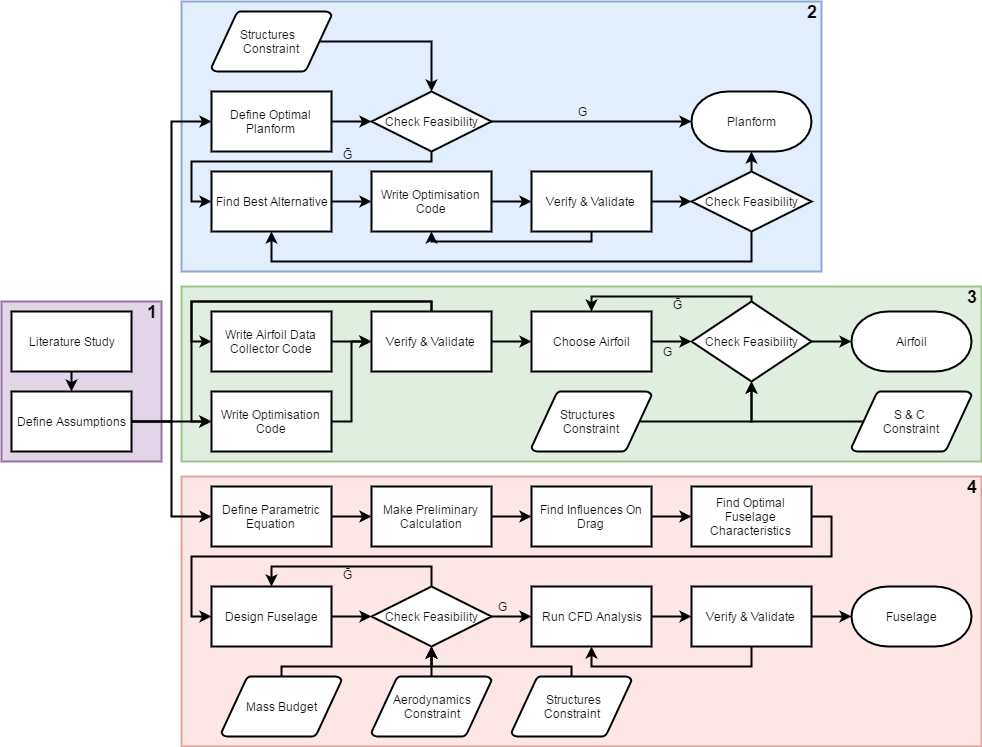
\includegraphics[scale=0.45]{Aerodynamics/Figures/Aerodynamic.png}
    \caption{Work Flow Diagram for the Aerodynamic Design Process}
    \label{fig:flow:aerodynamics}
\end{figure}

The work flow diagram shows four different coloured regions, these are the separate processes that have been done, though not only four processes have taken place. The first region is the general work needed before the designing can start. The literature study will help with understanding how to perform the design, and the assumptions will be made to give an overview how the design can be done. Once that is done, it is possible to go to any of the other regions based on what needs to be designed.

The second region contains the work flow diagram for the sizing and shape design of both the wing and the tail. The process for both these subsystems are very similar, hence they have the same work flow diagram. The first step of the process is to define the optimal planform shape, which would be the one to induce the least amount of drag. Once that is done, it needs to be checked if it is feasible with the constraints set by the structures department. If feasible, then the planform is done. If it is not feasible, a new best alternative has to be determined. With the help of a Python code the optimal alternative can be found, and again checked to be feasible. Now, if it is not feasible, the iteration starts to find the correct planform.

The third region is the work flow diagram for the airfoil selection for both the wing and the tail. Before this process can start, a code has to be written to collect all airfoil data and a code for the optimisation of the airfoils. Verification and validation will check if the code used it correct. Once all the data is collected and the optimisation made, the airfoil will be checked for feasibility, constrained by the structures department and the stability \& control department. If the airfoil turns out to be infeasible, a new airfoil optimisation will be run with new constraints to find the new best airfoil.

The fourth region is used for the design of the fuselage and the pylon. To start off the process, several parametric equations are selected, which are used to make preliminary calculations. Once the calculations are done, it is possible to find the major influences of drag of the fuselage. Knowing these influences, the optimal fuselage characteristics can be found, with which it is possible to design the fuselage. Once again, when the fuselage is designed, it needs to be checked for feasibility. This time the constraints come from the structures department, the aerodynamics department and the mass budget. If the design is feasible, a CFD (Computational Fluid Dynamics) analysis can be done to find more precise aerodynamic characteristics. The results of the CFD analysis is reflected against the parametric equations to check whether the CFD analysis has been implemented correctly.

\section{Assumptions}

\begin{itemize}
    \item The flight condition is assumed to be at an altitude of 120 meters. This has been chosen because the majority of missions will not be flown at higher altitudes, so it will be optimised for 120 meter altitude. CHECK EFFECTS LATER
    \item The increment in velocity due to the pusher props are assumed to be negligible, not affecting the wing aerodynamics. In reality they will increase the speed over the wing and decrease the amount of detached airflow, which increases the lift over the wing.
    \item The lifting surfaces are assumed to be completely smooth. In reality there are imperfections and other aspects, e.g. attachments, which decrease lift and increase drag.
    \item The drag of the propellers and motors are neglected. In reality they produce drag, but due to a lack of resources it was not possible to analyse this.
    \item The upwash and downwash of the wing on the pylons is neglected. In reality this effect would create a destabilising positive pitching moment. Nevertheless, ignoring this is acceptable as the pylons are narrow and the resulting pitching moment will be orders of magnitude smaller than the one created by the wing and tail.
    \item The pylon-fuselage interface is not analysed for aerodynamic influence. In reality, without implementing appropriate fairings, this interface is an additional source of parasitic drag. Nevertheless, at the current cruise velocities this drag is small in comparison with the other sources of drag and therefore may be neglected.
    \item It is assumed that for the fuselage CFD analysis the boundary layer is completely laminar. In reality, the boundary layer over the fuselage will transition to a turbulent flow. Yet it is assumed that the boundary layer will remain laminar along most of the length of the fuselage. This yields lower skin friction drag \cite[75]{anderson}, \cite[170]{fluidmech}.
\end{itemize}

\section{Analysis}

\subsection{Wing}

Introduction bout wing order etc

\subsection*{Shape \& Size}

\paragraph{Literature Study} For low speed aircraft, there is one major influence of drag on the wing, the induced drag. Seeming this UAV flies at low speeds (20-55 $\frac{m}{s}$), the induced drag will be the biggest source of drag on the wing. To minimise the drag, the lift distribution of the wing needs to be elliptical, which can be achieved by having an elliptical planform. This would be the optimum design of the wing, as shown in \autoref{fig:flow:shapeandsize}. However, an elliptical wing is harder to manufacture due to its complex shape \cite{ellipticalmanu}. Due to this, an alternative has to be found, which still resembles an elliptical lift the best. This can be done by using several taper ratio's or having a different airfoil at different spanwise locations. Due to the seeming complex manufacturing of different spanwise airfoils, the choice has been made to have several different tapers to resemble an elliptical lift distribution.

Another aspect of the planform which has been looked at is the sweep of the wing (or a front taper). Usually the front is swept to reduce mach bubbles being created on the wing, which reduces lift drastically and generates a lot of drag. But this effect occurs only at high speeds (M \textgreater 0.8) so it is not necessary for this UAV to have it. Having a swept wing will only have an adverse effect by reducing the speed over the airfoil, hence reducing lift. If the lift decreases, a bigger surface area will be needed which would only increase the drag.

\paragraph{Method} The sizing of the wing has been done by looking at the wing loading. The surface area needed to generate enough lift depends on various factors, see \autoref{eq:liftgenerate}.

\begin{equation}
    S = \frac{2W}{C_{L} V^2 \rho}
\end{equation}

Using airdensity at sea level and the stall speed of 20 $\frac{m}{s}$, it is possible to find the wing loading for different $C_{L}$ values. The best $C_{L}$, at a feasible wing loading, is 1.3. With this number the size of the planform is known, namely the surface area, which is 0.8 $m^2$.

Seeming the optimum solution, an elliptical planform, is not feasible, it is necessary to find the best alternative solution. With the choice to have several different taper ratio's, it has been chosen to use two different taper ratio's on the wing. This choice has been made seeming the wing has to be detachable for ground handling, so the location of the taper change will be where the wing is detachable. Having extra tapers would implicate the manufacturing while improving the planform slightly. 

To find the best planform, a python code has been made. The code has been made in such a way that it would iterate through most variables, which can be seen in REF, to find all possible combinations of planforms. Each planform generated has been compared to an elliptical planform, using the mean squared error of the differences of normalised chord lengths. This way the planform which resembles an ellipse the most could be chosen. To verify the planform for its elliptical lift, the program XFLR5 has been used, which can generate the lift of a 3D wing and show its distribution. The resulting lift distribution can be seen in \autoref{fig:liftdistribution}.

\paragraph{Results}

With the design process done, the planform of the wing had been finalised. The result can be seen in \autoref{fig:wingplanform}. The various dimensions of the planform are summarised in \autoref{tab:dimensionswing}.

\begin{figure}[H]
    \centering
    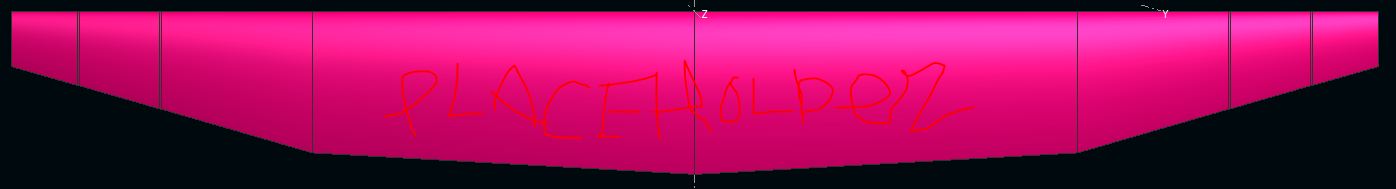
\includegraphics[scale=0.35]{Aerodynamics/Figures/Planform_Placeholder}
    \caption{Planform of the Wing}
    \label{fig:wingplanform}
\end{figure}

\begin{table}[H]
    \centering
    \begin{tabular}{ccc|ccc}
    Variable     &  Value & Iterated? & Variable & Value & Iterated?\\ \toprule
    $C_t$     & 118mm & Yes & $C_r$ & 348mm & Yes\\
    b & 2920mm & Yes & AR & 10.7 & No \\
    $\lambda_{tip}$ & 0.39 & Yes & $\lambda_{root}$ & 0.87 & No \\
    $l_{twist}$ & 146mm & Yes & $l_{taperchange}$ & 642mm & Yes
    \end{tabular}
    \caption{Dimensions of the Wing}
    \label{tab:dimensionswing}
\end{table}

\nomenclature[B]{$C_t$}{Tip chord \nomunit{m}}
\nomenclature[B]{$C_r$}{Root chord \nomunit{m}}
\nomenclature[B]{$b$}{Span \nomunit{m}}
\nomenclature[B]{$AR$}{Aspect Ratio \nomunit{-}}
\nomenclature[G]{$\lambda_{tip}$}{Taper ratio at tip \nomunit{-}}
\nomenclature[G]{$\lambda_{root}$}{Taper ratio at root \nomunit{-}}
\nomenclature[B]{$l_{twist}$}{Length of twist on wing (one side) \nomunit{m}}
\nomenclature[B]{$l_{taperchange}$}{Length where taper changes, as seen from the tip \nomunit{m}}
\nomenclature[B]{$C_L$}{Lift coefficient \nomunit{-}}

\subsection*{Airfoil}

\paragraph{Literature Study} It is possible to achieve lift employing various methods, one being the use of airfoils. These produce lift while minimising their drag contribution. Therefore it possible to achieve high efficiency, which in turn depends on the airfoil geometry. Airfoils are classified into families, and depending on which family the airfoil belongs to, different parameters are used to describe the geometry. Airfoils within one family will show similar shape characteristics, which also distinguish them from the other families. Since the aerodynamic performance is directly influenced by the shape, every airfoil family will therefore have distinct aerodynamic characteristics. Thus the application of the airfoil serves as the starting point for airfoil selection, starting with the selection of the airfoil family.

The most common airfoil families are the NACA 4-, 5-, and 6-digit series. The geometries of these airfoils are defined by the maximum camber value and position, the maximum thickness, and the family-specific parametric equations. Since the Hybrid UAV must be able to transition from horizontal to vertical flight, it is essential that the airfoil is predictable at low velocities and high angles of attack ensuring a safe transition. Therefore, the airfoil chosen for the Hybrid UAV must demonstrate gentle stall behaviour, which is true only with the NACA 4-digit series \cite{naca_series}. For this series, the first digit indicates the maximum camber, the second specifies the position of the maximum camber, and the last two digits indicate the maximum thickness of the airfoil. All these values are shown as a percentage of the chord.

Apart from the general aerodynamic behaviour, the airfoil's lift and drag (or $C_{L}$ and $C_{D}$) relationship must also be considered since it dictates the efficiency. In the case of the Hybrid UAV, two ratios are of greatest importance, namely $\frac{C_{L}}{C_{D}}$ influences the maximum range, and $\frac{C_{L}^{1.5}}{C_{D}}$ influences the maximum endurance \cite{perf}. Since the Hybrid UAV will mostly fly in cruise condition, the aim is to maximise both of these ratios for the lift coefficient required at cruise velocity, effectively yielding the optimal airfoil.

\paragraph{Method} The selection of the airfoil was done in two steps. Firstly, a list of all possible NACA 4-digit series airfoils was generated, with parameters ranging from 0008 to 5530. These were then inspected for their maximum lift coefficient and all airfoils which had a $C_{L,max}$ lower than 1.3 (dictated by the stall velocity) were discarded. 

The second step consisted of calculating the $\frac{C_{L}}{C_{D}}$ and $\frac{C_{L}^{1.5}}{C_{D}}$ at a $C_{L}$ value of 0.56 ($C_{L,cruise}$) for the remaining airfoils. Next, the airfoil with the highest $\frac{C_{L}}{C_{D}}$ ratio, and the airfoil with the highest $\frac{C_{L}^{1.5}}{C_{D}}$ ratio was found, yielding two airfoils optimised either for maximum range, or maximum endurance.

\paragraph{Results} 

\subsection*{High Lift Devices}

\paragraph{Literature Study} High lift devices are necessary in aircraft to be able to fly at lower stall speeds, seeming the high lift devices increase the $C_{L}$ of the wing. This comes in handy for large aircraft, so that the landing speed can be reduced significantly, ensuring a safer landing. However, this design does not need to land horizontally, meaning that this is not a problem. High lift devices can still be implemented to be able to ensure a lower stall speed, but adding high lift devices brings forward more disadvantages than advantages. They will increase the overall cost of the aircraft due to extra material cost and manufacturing costs and it brings complexity in the wing which is unnecessary. More loads will be introduced, hence more structural integrity will be needed. These factors alone are the reason why the choice has been made not to use high lift devices.

\subsection*{3D Wing}

\subsection*{Wingtips}

\paragraph{Literature Study} Wingtips decrease the drag of a wing by reducing the force of the tip vortices. This means the efficiency of the plane increases when using wingtips, although the factor it increases is too low to consider for this design. Having the improved efficiency from the winglets does not overcome the disadvantages it brings with it. Having winglets increases the overall cost due to extra material for the surface and the internal structures (more wing loading). Seeming the efficiency gained is not worth it, it has been decided not to use winglets.

\subsection{Tail}

\subsection*{Shape}

\paragraph{Literature Study} There are two parts of the tail which need to be shaped and sized, the horizontal and the vertical tail. The empennage will be a T-tail type, chosen by the stability and control department. This means that the vertical tail will be closed in by the horizontal tail and the fuselage. Due to this, the vertical tail has been shaped in such a way that it would just fit between these two other parts of the aircraft. The horizontal tail however, has been shaped to minimise the drag. Just as for the wing, the minimal drag occurs when there is an elliptical lift distribution. This time, it is possible to achieve this, due to three reasons. The first reason being that the loads on the horizontal tailplane are low, meaning the inner structure can be small and less complex. Furthermore, the size of the tailplane is a lot smaller than that of the wing, easing the manufacturing. The last reason is that the tailplane is not as complex as the wing. Due to these reasons the horizontal tailplane has been chosen to have an elliptical lift distribution.

\paragraph{Approach} The key to getting a elliptical lift distribution is to have the chord lengths follow the size of an ellipse, although the centre of the ellipse can be moved around. Keeping in mind that the elevators are most efficient if perpendicular to the flow, the horizontal centre line of the planform has been moved down to the quarter-chord point. This way the elliptical lift distribution is kept while having more controllability with the elevators. 

Having an elliptical lift distribution does not say anything about the root chord and span of the tailplane, so to size these dimensions reference aircraft have been used. The usual aspect ratios of horizontal and vertical tailplanes are about 5. With this value, and the surface areas acquired from the stability \& control department, the final dimensions could be calculated for both the vertical and horizontal tailplane.


\paragraph{Results} With the shaping done, it is possible to find the dimensions of the wing.

\subsection*{Airfoil}

\subsection{Fuselage}

\subsection{Pylon}

\section{Verification \& Validation}

\section{Results}




%%%%%%%%%%
%%%%%%%%%%
%%%%%%%%%%

\begin{comment}

\section{Wing}

There are several departments that have worked on the design of the wing, these are the aerodynamics department, the stability \& control department and the structures department. The aerodynamics departments has taken a look into various aspects of the wing, starting with the shape and size of the wing, e.g. the wing planform. When the planform of the wing was designed, the airfoil could be chosen. With the most important aerodynamic aspects of the wing chosen, it was possible to look into the possibility to have winglets or high lift devices.

%Aerodynamics from here
\subsection{Aerodynamics}

\subsection*{Shape \& Size}

The shape and size of the wing will alter the aerodynamic properties of the wing, e.g. an increase in drag or a decrease in lift. Choosing the best wing planform will be crucial in order to be able to fulfil all the requirements. \autoref{fig:flow:shapeandsize} shows the process needed to come up with the best wing planform.

\begin{figure}[H]
    \centering
    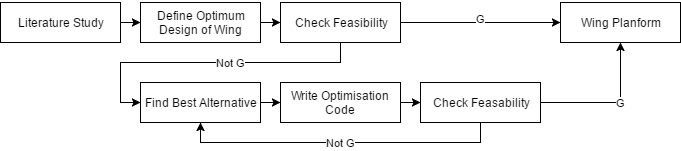
\includegraphics[scale=0.6]{WingTail/Figures/shapeandsize2}
    \caption{Work Flow Diagram for Wing Sizing and Shape}
    \label{fig:flow:shapeandsize}
\end{figure}

The first step will be to do some literature study about the subject, finding what is most crucial to coming up with a wing planform. When that is done, the optimum wing design will be defined, according to that literature study. Once that is done it will need to be check for feasibility, it could be constrained due to mass or cost, or due to one of the other departments. If it is feasible, then the wing planform has been defined; if not, then another solution must be made. An optimisation code will be written to find the best alternative which could fulfil the requirements and not be constrained by other factors. Each time the alternative will be checked if feasible.



\end{comment}

%%%%%%%
